% Template for Elsevier CRC journal article
% version 1.1 dated 16 March 2010

% This file (c) 2010 Elsevier Ltd.  Modifications may be freely made,
% provided the edited file is saved under a different name

% This file contains modifications for Procedia Computer Science
% but may easily be adapted to other journals

% Changes since version 1.0
% - elsarticle class option changed from 1p to 3p (to better reflect CRC layout)

%-----------------------------------------------------------------------------------

%% This template uses the elsarticle.cls document class and the extension package ecrc.sty
%% For full documentation on usage of elsarticle.cls, consult the documentation "elsdoc.pdf"
%% Further resources available at http://www.elsevier.com/latex

%-----------------------------------------------------------------------------------

%%%%%%%%%%%%%%%%%%%%%%%%%%%%%%%%%%%%%%%%%%%%%%
%%%%%%%%%%%%%%%%%%%%%%%%%%%%%%%%%%%%%%%%%%%%%%
%%                                          %%
%% Important note on usage                  %%
%% -----------------------                  %%
%% This file must be compiled with PDFLaTeX %%
%% Using standard LaTeX will not work!      %%
%%                                          %%
%%%%%%%%%%%%%%%%%%%%%%%%%%%%%%%%%%%%%%%%%%%%%%
%%%%%%%%%%%%%%%%%%%%%%%%%%%%%%%%%%%%%%%%%%%%%%

%% The '3p' and 'times' class options of elsarticle are used for Elsevier CRC
\documentclass[3p,times]{elsarticle}

%% The `ecrc' package must be called to make the CRC functionality available
%\usepackage{ecrc}

%% The ecrc package defines commands needed for running heads and logos.
%% For running heads, you can set the journal name, the volume, the starting page and the authors

%% set the volume if you know. Otherwise `00'
%\volume{00}

%% set the starting page if not 1
%\firstpage{1}

%% Give the name of the journal
%\journalname{}

%% Give the author list to appear in the running head
%% Example \runauth{C.V. Radhakrishnan et al.}
%\runauth{}

%% The choice of journal logo is determined by the \jid and \jnltitlelogo commands.
%% A user-supplied logo with the name <\jid>logo.pdf will be inserted if present.
%% e.g. if \jid{yspmi} the system will look for a file yspmilogo.pdf
%% Otherwise the content of \jnltitlelogo will be set between horizontal lines as a default logo

%% Give the abbreviation of the Journal.
%\jid{procs}

%% Give a short journal name for the dummy logo (if needed)
%\jnltitlelogo{}

%% Hereafter the template follows `elsarticle'.
%% For more details see the existing template files elsarticle-template-harv.tex and elsarticle-template-num.tex.

%% Elsevier CRC generally uses a numbered reference style
%% For this, the conventions of elsarticle-template-num.tex should be followed (included below)
%% If using BibTeX, use the style file elsarticle-num.bst

%% End of ecrc-specific commands
%%%%%%%%%%%%%%%%%%%%%%%%%%%%%%%%%%%%%%%%%%%%%%%%%%%%%%%%%%%%%%%%%%%%%%%%%%

%% The amssymb package provides various useful mathematical symbols
\usepackage{amssymb}
%% The amsthm package provides extended theorem environments
\usepackage{amsthm}
\usepackage{amsmath}
%% The lineno packages adds line numbers. Start line numbering with
%% \begin{linenumbers}, end it with \end{linenumbers}. Or switch it on
%% for the whole article with \linenumbers after \end{frontmatter}.
%% \usepackage{lineno}

%% natbib.sty is loaded by default. However, natbib options can be
%% provided with \biboptions{...} command. Following options are
%% valid:

%%   round  -  round parentheses are used (default)
%%   square -  square brackets are used   [option]
%%   curly  -  curly braces are used      {option}
%%   angle  -  angle brackets are used    <option>
%%   semicolon  -  multiple citations separated by semi-colon
%%   colon  - same as semicolon, an earlier confusion
%%   comma  -  separated by comma
%%   numbers-  selects numerical citations
%%   super  -  numerical citations as superscripts
%%   sort   -  sorts multiple citations according to order in ref. list
%%   sort&compress   -  like sort, but also compresses numerical citations
%%   compress - compresses without sorting
%%
% \biboptions{comma,round}

 \biboptions{compress}
\usepackage{color}
\def\red#1{{\color{red}{#1}\color{black}}}
% if you have landscape tables
\usepackage[figuresright]{rotating}
\usepackage{amssymb}
% put your own definitions here:
%\newcommand{\eqref}{Ref.}
%   \newtheorem{def}{Definition}[section]
%   ...
\newfont{\fp}{msbm10 at 11pt}  
\def\E{\mbox{\fp E}}
\def\proof{\mbox{\fp Proof:}}
\newtheorem{prop}{Proposition}
\newtheorem{thm}{Theorem}
\usepackage[T1]{fontenc}
\usepackage{amsfonts}
\newtheorem{lem}{Lemma}
% add words to TeX's hyphenation exception list
%\hyphenation{author another created financial paper re-commend-ed Post-Script}

% declarations for front matter

\usepackage{color, colortbl, framed}

\begin{document}

\begin{frontmatter}

%% Title, authors and addresses

%% use the tnoteref command within \title for footnotes;
%% use the tnotetext command for the associated footnote;
%% use the fnref command within \author or \address for footnotes;
%% use the fntext command for the associated footnote;
%% use the corref command within \author for corresponding author footnotes;
%% use the cortext command for the associated footnote;
%% use the ead command for the email address,
%% and the form \ead[url] for the home page:
%%
%% \title{Title\tnoteref{label1}}
%% \tnotetext[label1]{}
%% \author{Name\corref{cor1}\fnref{label2}}
%% \ead{email address}
%% \ead[url]{home page}
%% \fntext[label2]{}
%% \cortext[cor1]{}
%% \address{Address\fnref{label3}}
%% \fntext[label3]{}

%\dochead{}
%% Use \dochead if there is an article header, e.g. \dochead{Short communication}
\title{Selection of informative frequency band in local damage detection in rotating machinery}

%% use optional labels to link authors explicitly to addresses:
%% \author[label1,label2]{<author name>}
%% \address[label1]{<address>}
%% \address[label2]{<address>}

\author{Jakub Obuchowski\fnref{label1}}
  %\ead{jakub.obuchowski@pwr.wroc.pl}
 % \tnotetext[label2]{}
\author{Agnieszka Wy{\l}oma{\'n}ska\fnref{label2}}
 %\ead{agnieszka.wylomanska@pwr.wroc.pl}
 %\tnotetext[label3]{}
   \author{Rados{\l}aw Zimroz\fnref{label1}}
  %  \ead{radoslaw.zimroz@pwr.wroc.pl}
%% \ead[url]{home page}\fntext[label2]{}
   \fntext[label1]{Diagnostics and Vibro-Acoustics Science Laboratory, Na Grobli 15, 50-421 Wroclaw, Wroclaw University of Technology, PL\\jakub.obuchowski@pwr.wroc.pl. radoslaw.zimroz@pwr.wroc.pl}
  \fntext[label2]{Hugo Steinhaus Center, Institute of Mathematics and Computer Science, Janiszewskiego 14 a, 50-370 Wroclaw, Wroclaw University of Technology, PL\\
   agnieszka.wylomanska@pwr.wroc.pl}

\begin{abstract}
Problem of informative frequency band (IFB) selection in vibration signal processing for local damage detection is discussed. It is proposed to extend the concept of automatic and objective IFB selection proposed by several authors. Till now, kurtosis was preferred as criterion for IFB search. Thus, it is offered to study set of statistics, namely Jarque-Bera, Kolmogorov-Smirnov, Cramer-von Mises, Anderson-Darling, quantile-quantile plot and a method based on the local maxima approach in order to verify their abilities of IFB selection. Also similarities between them are described. It has been proved by simulation and real data analysis that proposed selectors (because they allow us to "select" frequency band) might be equivalent to the spectral kurtosis (SK) in ordinary cases. Moreover, some of the novel selectors are better, because they are less sensitive to incidental spikes that might occur during the signal acquisition process. Proposed selectors might be (as SK) the basis for filter design for informative signal extraction.
\end{abstract}
\begin{keyword}

%% keywords here, in the form: keyword \sep keyword

%% MSC codes here, in the form: \MSC code \sep code
%% or \MSC[2008] code \sep code (2000 is the default)
local damage\sep vibration\sep time--frequency analysis \sep statistical analysis\sep band selector
\end{keyword}
\end{frontmatter}
\section{Introduction}
Local damage detection is one of the most widely explored problems in modern condition monitoring. One might notice two serious reasons of that. First, detection of such damage in industrial reality might be practically difficult due to poor signal to noise ratio and specific properties of informative signal. Second, localized damage causes significant, local increase of interaction of surfaces being in contact. It means that at these time moments forces/moments are several (or more) times bigger than during normal operation. It accelerates degradation and might rapidly (much quicker than distributed damage) cause catastrophic failure. Vibration analysis seems to be the most effective approach for this problem. Mechanism of generation of informative signals is well recognized~\cite{bib13,bib18,bib19,bib36}. Local change of stiffness associated with crack or loss of surface causes impulsive disturbance in the signal. Due to rotation of elements, these disturbances should be cyclic. In simple case, these impulses are visible in time domain and basic techniques might be effective enough to detect damage. Next step after detection is association of damage with particular element with predefined (based on design factors and operating conditions), so called characteristic frequencies. Motivation of advanced study for local damage detection is provided by industrial signals from machines with complexity of design, corruption of signals by significant noise or early stage of damage. In such industrial case, mentioned cyclic pulse train might be hardly seen. One needs to "extract" informative signal from mixture of signals coming from different sources. By "noise" in such context one might consider discrete component coming from shaft, mesh, resonance, ghost, etc. components, wideband Gaussian noise, or other. The most reasonable approach is to design a filter that would be able to extract the signal of interest (SOI).\\
The key issue is a data-driven filter design procedure. It is known that filter can be described by its impulse response in time domain or transfer function (amplitude and phase characteristics) in frequency domain. In the second approach one has to specify which frequencies are informative (should be passed without changes) and non-informative (should be suppressed). Knowledge about location of informative frequency bands might allow to use simple band-pass filter, wavelet filter, so called Wiener filter, etc.  How to find the signal of interest? How to find frequency bands where signal of interest after filtering is clearly visible? In the paper we propose solutions to these problems.\\
The rest of the paper is organized as follows: in Sec.~\ref{state} we briefly review works which are strictly connected to the subject of this paper. In Sec.~\ref{selectors} a proposal of new frequency band selectors is presented. Sec.~\ref{simulation} contains analysis of simulated data according to the presented procedure. In Sec.~\ref{real} we present the results for the real industrial data. Last section contains conclusions.
\section{State of the art}\label{state}
A signal that represents local damage is often amplitude or frequency modulated by AM or FM phenomena, thus we incorporate the concept of IFB defined as a frequency band with carrier frequency as the center frequency and the bandwidth that depends on modulation depth. The key question is to find the carrier and the bandwidth. The carrier is related to mesh frequencies or resonance frequencies. The idea of signal filtering and further demodulation around structural resonance was  described in~\cite{bib13} (for bearings) and~\cite{bib39} (for gears). It is known that for resonance area signal is enhanced "naturally" by resonance related amplification.\\
In Authors' belief, the work proposed by Lin and Zuo in~\cite{bib40} is in some sense a breakthrough in automatic determining of informative frequency band. They proposed an adaptive wavelet filter based on Morlet wavelet. The Morlet wavelet parameters optimization scheme was proposed with the kurtosis as maximization principle. It has been shown that in a set of scale parameters and $\beta$ parameters of daughter Morlet wavelet the kurtosis value is significantly higher for parameters chosen by that scheme. It means that for such shape of wavelet, the results of filtering are the most impulsive, which leads to conclusion about the highest visibility of damage. In fact, this approach is in some sense extended in other works.\\
There is a collection of papers where the authors try to optimize or adapt wavelet based filtering~\cite{bib41,bib42,Bozchalooi,bib43,bib44,Tse2,bib45}. In~\cite{bib41} authors use a complex shifted Morlet wavelet family for demodulation. Authors of~\cite{bib42} proposed a novel wavelet transform called exact wavelet analysis which design is based on genetic algorithms. The method minimizes the undesirable effect of overlapping and makes it easier to detect faults and distinguish the causes of faults. Bozchalooi and Liang~\cite{Bozchalooi} introduced a smoothness index defined as the ratio of the geometric mean to the arithmetic mean of the wavelet coefficient moduli of the vibration signal. It guides to select proper wavelet parameters. In~\cite{bib43} a method of impulsive features extraction in the vibration signal is proposed which combines Morlet wavelet filter and sparse code shrinkage (SCS). Another usage of Morlet wavelet is presented in~\cite{bib44} where authors use it to determine a bandpass filter to eliminate the frequency related to interferential vibrations. Then an autocorrelation enhancement algorithm is applied to obtain a signal with only few spectral lines remained. In a two-part work done by Tse and Wang~\cite{Tse2,bib45} a new sparsogram is introduced. It quickly determines the resonant frequency bands which contain information about damage.\\
Another idea that influenced researches was introduced to condition monitoring community by Antoni in~\cite{bib20}. He proposed to apply the kurtosis for sub-signals taken from spectrogram for each frequency bin, i.e. spectral kurtosis  as a statistical tool which can indicate the presence of series of transients and their locations in the frequency domain. It might be calculated using time-frequency map and point out these frequency bins on time-frequency map, that reveal the most  impulsive nature. Extension of this approach and practical implementation was presented by Antoni and Randall in~\cite{bib23}.
Antoni proposed also dyadic signal decomposition scheme, that also uses kurtosis to select frequency band. The approach was called kurtogram.  Further extension and application of SK and kurtogram might be found in many papers~\cite{bib24,bib46,bib47,bib48,bib49}. 
It is worth mentioning that Zhang and Randall~\cite{bib49} proposed kurtogram with genetic algorithm based optimization, Wang and Liang~\cite{bib46} proposed an adaptation scheme for SK and Lei et al.~\cite{bib48} adapted wavelet packet transform (WPT) for kurtogram. Wang et al.~\cite{bib47} proposed an enhanced kurtogram, with kurtosis values calculated based on the power spectrum of the envelope of the signals extracted from wavelet packet nodes at different depths. Barszcz and Jab{\l}o{\'n}ski~\cite{bib25}  proposed a technique called the protrugram  that is based on kurtosis of the envelope spectrum amplitudes of the demodulated signal, instead of the kurtosis of the filtered time signal. They claim that the advantage of the method is the ability to detect transients with smaller signal-to-noise ratio comparing to the SK--based fast kurtogram.\\
Urbanek et al.~\cite{bib27} has proposed a novel technique called modulation intensity distribution for  estimation of informative frequency band. The basic assumption is that local damage produces non-linear phenomena that might be modeled as amplitude modulation. If in the bi-frequency plane a non-zero component with frequency corresponding to a carrier and a sideband is present, it means that the carrier and the sideband are correlated and the frequency band is informative. Makowski and Zimroz~\cite{bib28} proposed a procedure based on statistical analysis of parametric time-frequency map that allows to extract set of informative bands and further processing of energy flow at these ranges. Obuchowski et al.~\cite{bib29}  introduced a family of statistical criteria that might be used instead of kurtosis for informative frequency band search.\\
It should be said that there are other possible approaches that might provide serious signal enhancement without pre-defining frequency band as EMD~\cite{bib33,bib50} or adaptive filters~\cite{bib18,bib32,bib35,bib30}. In both cases, proposed procedures do not specify any particular frequency band, it is adaptively obtained depending on data (data-driven filters).
\section{Informative frequency band selectors}\label{selectors}
In this section we introduce the novel procedure that leads to the local damage detection in rotating machinery. This procedure is based on the time-frequency representation of examined signal. More precisely, in the first step of our analysis we decompose the signal into set of narrowband sub-signals using a time-frequency representation. Here we propose to use the short-time Fourier transform (STFT) that  is defined as follows~\cite{allen}:
\begin{eqnarray}\label{stft1}
STFT(t,f)=\int_{-\infty}^{\infty}{w(t-\tau)X(\tau)e^{2j\pi f\tau}}\, \mathrm{d} \tau,
\label{stft-cont}\end{eqnarray}
where $w(t-\tau)$ is the shifted window and $X(\tau)$ is the input signal. Discrete version of equation~(\ref{stft1}) for observations $X_1,X_2,...,X_N$, time point $t\in T$ and frequency $f\in \textit{F} $ is defined as follows:
\begin{eqnarray}
STFT(t,f)=\sum_{k=0}^{N-1}X_k w(t-k)e^{2j\pi f k/N}.
\label{stft-discr}\end{eqnarray}
In the second step of our analysis we use several statistics, called selectors, that can be useful as tools for assessment of the sub-signals. Each sub-signal is slice for a given narrow frequency range that arises after mentioned time-frequency decomposition. In this paper we extend the classical approach, where the kurtosis of sub-signals is calculated and propose new selectors based on statistical properties of examined sub-signals. The primary analysis of rotating machinery indicates that sub-signals related to machine in healthy condition are closer to Gaussian than sub-signals related to a damaged one, so some of the proposed statistics are based on the distance between empirical distribution of examined sub-signal and the base distribution, namely the Gaussian one. The selectors mentioned in this paper might be grouped with respect to their statistical properties. In the following subsections we describe the selectors grouped with respect to their statistical properties.
\subsection{Moment-based selectors}
One of the most popular selectors that might be applied to local damage detection of underlying signal is the spectral kurtosis ($SK$),~\cite{bib23}. The spectral kurtosis  was first introduced as a statistical tool which can indicate not only non-Gaussian components in a signal, but also their locations in the frequency domain. The spectral kurtosis at the frequency band $f$ is defined as follows~\cite{bib23}:
\begin{eqnarray}\label{spectral_kurtosis}
SK(f)=\#T\frac{\sum_{t\in T}|STFT(t,f)|^4}{(\sum_{t\in T}|STFT(t,f)|^2)^2}-2,
\end{eqnarray}
where $\#T$ denotes the number of elements of the set $T$, i.e. number of time points at which STFT is calculated.\\
Since the spectral kurtosis is based on the fourth-order moment, this group of selectors will be complemented with a statistic which is based on both fourth and third moment, namely the Jarque-Bera ($JB$) statistic. It is strictly related to the Jarque-Bera test, which is a goodness-of-fit test of whether sample data has the skewness and kurtosis matching a Gaussian distribution. This methodology is an extension of the  widely used scheme where only the empirical kurtosis is being investigated. The $JB$ statistic calculated for sub-signal corresponding to frequency band $f$ is defined as:
\begin{eqnarray}
JB(f)=\frac{\#T}{6}\left(S(f)^2+\frac{\left(K(f)-1\right)^2}{4}\right),
\end{eqnarray}
where $S(f)$ and $K(f)$ are the empirical skewness and kurtosis, respectively, calculated for given sub-signal corresponding to frequency band $f$.\\
The value of the $JB$ statistic forms a random variable which converges to zero if the underlying distribution has skewness zero and kurtosis 3 (e.g. Gaussian). Any deviation from zero skewness and kurtosis equal to 3 increases the $JB$ statistic.  In this paper the $JB$ statistic is one of the proposed selectors used for local damage detection. If the data come from Gaussian distribution, the $JB$ statistic asymptotically has a chi-squared distribution with two degrees of freedom, so the statistic can be used to test the hypothesis that the data are derived from a Gaussian distribution. The null hypothesis is a joint hypothesis of the skewness being zero and the excess kurtosis being zero. As the definition of $JB$ shows, any deviation from these values increases the $JB$ statistic.\\
\subsection{ECDF-based selectors}
In this section we describe selectors based on the empirical cumulative distribution function (ECDF). The fundamental statistical property of them is that, for specific distributions, moments of a random variable might be infinite, while cumulative distribution function is always well-defined. Moreover, these two groups are different from the computational point of view - calculating ECDF requires sorting of the sample.\\
The first proposed selector in this group is a Kolmogorov-Smirnov  statistic ($KSS$) that for sub-signal corresponding to the frequency band $f$ is defined as follows~\cite{bib03,bib04}:
\begin{eqnarray}\label{K-S}
KSS(f)=sup_x\left|ECDF(f,x)-\Phi(f,x)\right|,
\end{eqnarray}
where $\Phi(f,\cdot)$ is the cumulative distribution function of the Gaussian distribution with parameters estimated from the sub-signal corresponding to the frequency band $f$. Therefore this function is given by:
\begin{eqnarray}\label{FF}\Phi(f,x)=\int^{x}_{-\infty} \! \frac{1}{\sqrt{2\pi\widehat{\sigma(f)}^2}}\exp \left( -\frac{\left(x-\widehat{\mu(f)}\right)^2}{2\widehat{\sigma(f)}^2} \right) \, \mathrm{d} x,\end{eqnarray}
where $\widehat{\mu(f)}$ is the empirical mean of the sub-signal $\{|STFT(t,f)|\}_{t\in T}$, and $\widehat{\sigma(f)}$ is the empirical standard deviation of  $\{|STFT(t,f)|\}_{t\in T}$. Moreover $ECDF(f,x)$ is the empirical cumulative distribution function calculated for the sub-signal corresponding to the frequency band $f$:
\begin{eqnarray}\label{ECDF}
ECDF(f,x)=\frac{1}{\#T}\sum_{t\in T}\mathbf{1}\left\{ |STFT(t_k,f)|\leq x\right\}
\end{eqnarray}
In the above definition $\mathbf{1}\{A\}$ denotes the indicator of the set A.\\
\begin{figure}[!ht]
\begin{center}
\includegraphics[width=0.4\textwidth]{fig01aecdf_g.eps}
\includegraphics[width=0.4\textwidth]{fig01becdf_b.eps}
\caption{The empirical and theoretical (Gaussian) cumulative distribution functions for exemplary sub-signals from machine in good condition (left panel) and damaged one (right panel). The black dashed line represents the reference cumulative distribution function of Gaussian distribution.}\label{fig1}
\end{center}
\end{figure}
The idea of using the Kolmogorov-Smirnov statistic for spikiness detection is illustrated in Fig.~\ref{fig1}, where we present the empirical and theoretical cumulative distribution functions for real data set analyzed in Sec.~\ref{bearing}. In the left panel of Fig.~\ref{fig1} we show the cumulative distribution functions (empirical and theoretical - Gaussian) for sub-signal corresponding to the frequency $f=2325$~Hz for machine in good condition while in the right panel for the damaged one. One can observe in the left panel the analyzed functions are closer than in the right panel, therefore the $KSS$ for this frequency band has lower value for the sub-signal from machine in good condition. In~\cite{bib05,bib06} one can find more properties of the $KSS$ statistic and statistical test based on it. We only mention here the $KSS$ statistic tends to zero (almost surely) when number of elements in set $T$ tends to infinity. Moreover the distribution of $KSS$ statistic defined in (\ref{K-S}) is normal. The first fact is a result of Glivenko-Cantelli theorem~\cite{gli} while the second one is so called the distribution-free property.\\
The next statistic that might be a useful tool for informative band selection is an extension of the mentioned Kolmogorov-Smirnov. Similar to $KSS$, it is based on the distance between theoretical and empirical cumulative distribution functions for underlying sub-signal. The selector, called Anderson-Darling statistic, belongs to the Cramer-von Mises family of statistics which incorporate the idea of quadratic norm. The Cramer-von Mises statistic for frequency band $f$ is defined by~\cite{bib06}
\begin{eqnarray}
Q(f)=\#T\int^{\infty}_{-\infty} \! \left(ECDF\left(f,x\right) - \Phi\left(f,x\right)\right)^2 \phi \left(x\right) \, \mathrm{d} x
\end{eqnarray}
where $\phi \left(x\right)$ is a suitable function which puts weights to the squared difference $\left(ECDF\left(f,x \right) - \Phi\left(f,x\right)\right)^2$. Moreover functions $ECDF(f,x)$ and $\Phi(f,x)$ are defined in (\ref{FF}) and (\ref{ECDF}), respectively. When $\phi(x)=1$, $Q(f)$ is called the Cramer-von Mises statistic. In this case we denote it as $CVM$. If $\phi\left(x\right)=\left[ \Phi\left(f,x\right) \left( 1-\Phi\left(f,x\right) \right) \right]^{-1}$, the above definition yields the Anderson-Darling statistic.  In the further analysis it is denoted as $AD$. Similarly to the Kolmogorov-Smirnov statistic there exist statistical tests that allow to test the proper distribution of examined data by using the $CVM$ and $AD$ statistics. More details can be found in~\cite{bib07,bib08,bib09}. The Cramer-von Mises test has better properties than the Kolmogorov-Smirnov test, but has some disadvantages. In order to extend the $CVM$ test the Anderson-Darling test was introduced. The Anderson--Darling test is a statistical test of whether a given sample of data is drawn from a given probability distribution. In our case the base distribution is Gaussian. The test is one of the most powerful statistical tools for detecting deviations from gaussianity.\\
\subsection{Quantile-quantile plot-based selectors}
Except of statistical tests with explicit hypothesis, there are some visual tests to compare two distributions, e.g. the theoretical distribution and the empirical one. One of the most famous examples is the quantile-quantile plot (QQplot),~\cite{bib11}. Plot of the theoretical distribution quantiles versus the underlying ones might be useful to recognize goodness-of-fit. Straight line on the QQplot means that compared distributions have the same shape. Straight line with equal scales on the axes means equal distributions. If there is no straight line, then one can compare, for example, tail heaviness of both distributions. In most of numerical packages (MATLAB, R) there is an additional straight line plotted to make analysis easier. This line connects two points: first and third quartiles of both distributions. To make this test numerical, we propose to measure the horizontal distance between the QQplot markers and the additional straight line. One can note that statistics contained in this group require sorting, similar to the previous group. Nevertheless, the lack of explicit hypothesis of gaussianity test based on the QQplot tends us to classify them into an individual group.\\
\begin{figure}[!ht]
\begin{center}
\includegraphics[width=0.4\textwidth]{fig02aqqplot_g.eps}
\includegraphics[width=0.4\textwidth]{fig02bqqplot_b.eps}
\caption{QQplot of the healthy (left panel) and unhealthy (right panel) sub-signal compared to the normal distribution. The black dashed line represents the reference quantile line for Gaussian distribution. Note that only horizontal distance between markers and line is quantified by $H_{aver}$ and $H_{max}$.}\label{fig2}
\end{center}
\end{figure}
For this test, we propose to compute mean and maximum of those distances. The formula for the maximum distance between the Gaussian distribution and the sub-signal corresponding to the frequency band $f$ is as follows:
\begin{eqnarray}
H_{max}(f)=\max_{1\leq k \leq \#T}{ \left| \widetilde{\Phi}^{-1}\left(\frac{2k-1}{2\#T} \right) - a S(k,f)-b \right| },
\end{eqnarray}
where $\widetilde{\Phi}^{-1}(\cdot)$ is the inverse of cumulative distribution function of standard Gaussian distribution, i.e. $$\widetilde{\Phi}(x)=\int^{x}_{-\infty} \! \frac{1}{\sqrt{2\pi}}\exp \left( -\frac{x^2}{2} \right) \, \mathrm{d} x,$$ 
$S(k,f)$ is the $k$-th value of ascending sorted sub-signal $\{|STFT(t,f)|\}_{t\in T}$, $a=\dfrac{\widetilde{\Phi}^{-1}(0.75)-\widetilde{\Phi}^{-1}(0.25)}{q(f,0.75)-q(f,0.25)}$, $b=\widetilde{\Phi}^{-1}(0.75)-aq(f,0.75)$ and $q(f,p)$ is a $p$-th order quantile of a sub-signal $\{|STFT(t,f)|\}_{t\in T}$. The formula for the average distance is analogous with the $\max$ function substituted by the arithmetic mean. We denote the corresponding statistic as $H_{aver}$. The exemplary QQplots  for real data examined in Sec.~\ref{bearing} of a healthy signal (for a given frequency bin) is presented in Fig.~\ref{fig2} (left panel) while for the sub-signal with defect - in the right panel of Fig.~\ref{fig2}. We observe the healthy signal is closer to Gaussian distribution than the unhealthy one. Both average and maximum horizontal distances between straight line and markers are significantly larger in the right panel.
\subsection{Local maxima method-based selector}
The last procedure that allows for construction of a selector for local damage detection is based on the local maxima method~\cite{bib12,LMM}. For each frequency band (i.e. each sub-signal) we check the local maximum occurrence. We assume that local maximum occurs at a given time point when the modulus of STFT value therein is higher than the other values in its neighborhood of a length not less than a certain value - $r$. Then, for each frequency band we create a new binary vector which is a transformation of the original data into zero-one series. More precisely, we put 1 at a time point when the local maximum occurs and 0 otherwise. Let us point that the binary values obtained in this way minimize influence of insignificant signals for local damage detection as well as maximize influence of characteristic signals for locally damaged machinery. In our methodology for each time point we use the vector of weights (VoW), which is a vector of averaged maxima occurrence, i.e. VoW at point $t$ is defined as follows:
\begin{eqnarray}
W(t)=\frac{1}{\#\textit{F}}\sum_{f\in\textit{ F}}M(t,f),
\end{eqnarray}
where $M(t,f)$  represents binary valued vector of the local maxima occurrence at the time point  $t$ and frequency $f$. After multiplying each previously computed binary value by the value of VoW at the corresponding time point we obtain an enhanced spectrogram. Therefore the enhanced spectrogram at point $(t,f)$ is defined as follows:
\begin{eqnarray}
ENH(t,f)=W(t)M(t,f).
\end{eqnarray}
More details of the procedure for the enhanced spectrogram construction for different applications one can find in~\cite{bib12}. The selector based on the local maxima method for frequency band $f$ is constructed as follows:
\begin{eqnarray}
LM(f)=\frac{1}{\#T}\sum_{t\in T}ENH(t,f).
\end{eqnarray}
\section{Simulated data analysis}\label{simulation}
In this section we illustrate how the proposed selectors deal with simulated data set representing vibrations of hypothetical rotating machines, one of which is locally damaged and the second is in healthy condition. The signal $\left\{X(t)\right\}$ is obtained using the following formula:
\begin{eqnarray}
X(t)=\sum^{n}_{i=1}{ A a_i \sin(2\pi f_i t)} + \sigma N(t),
\end{eqnarray}
\begin{figure}[!ht]
\begin{center}
\includegraphics[width=0.7\textwidth]{sin_const-raw_signal_timeseries_g_noise.eps}
\includegraphics[width=0.7\textwidth]{sin_const-raw_signal_timeseries_b_noise.eps}
\caption{Signal of noise - $\left\{\sigma N(t)\right\}$ from healthy (top panel) and faulty (bottom panel) rotating machine. The whole signals last 2.5~s. Note some disturbations at 0.077, 0.15 and 0.23~s in bottom panel.}\label{1timeseries_noise}
\includegraphics[width=0.7\textwidth]{sin_const-raw_signal_timeseries_g.eps}
\includegraphics[width=0.7\textwidth]{sin_const-raw_signal_timeseries_b.eps}
\caption{Raw vibration signal from healthy (top panel) and faulty (bottom panel) rotating machine. The whole signals last 2.5~s. Note some barely-visible disturbations at 0.077, 0.15 and 0.23~s marked by ellipses.}\label{1timeseries}
\end{center}
\end{figure}
\begin{figure}[!ht]
\begin{center}
\includegraphics[width=0.7\textwidth]{sin_const-raw_signal_spectrogram_g.eps}
\includegraphics[width=0.7\textwidth]{sin_const-raw_signal_spectrogram_b.eps}
\caption{Spectrograms of raw vibration data from healthy (top panel) and faulty (bottom panel) rotating machine. The whole signals last 2.5~s. Note energy difference between low-frequency deterministic components and noise.}
\label{1spectrograms}
\end{center}
\end{figure}
where $n=6$, $A=10$, $a_i=0.75^{(i-1)}$, $f_i=190i$, $\sigma=0.1$ and $\left\{N(t)\right\}$ is white standard Gaussian noise in case of healthy machine. In case of local damage $\left\{N(t)\right\}$ is divided by filtering into 3 groups: a) $\left\{N_1(t)\right\}$ - lowpass filtered $\left\{N(t)\right\}$ with cut-off frequency 1000~Hz, b) $\left\{N_2(t)\right\}$ - bandpass filtered $\left\{N(t)\right\}$ with cut-off frequencies 1000~Hz and 6000~Hz and c) $\left\{N_1(t)\right\}$ - highpass filtered $\left\{N(t)\right\}$ with cut-off frequency 6000~Hz. We use ideal filters, i.e. filters with characteristics equal to 1 along the passed band and 0 elsewhere. To simulate the pulse train we modulate amplitude of $\left\{N_2(t)\right\}$ using an impulsive signal - sum of a lot of sine waves with frequencies that are multiples of the fault frequency. Amplitude of the result is adjusted to make level of noise between pulses similar to the level of $\left\{N(t)\right\}$ in healthy case.  Signal to noise ratio defined as $\mathrm{SNR_{dB}} = 10 \log_{10} \left ( \frac{P_\mathrm{signal}}{P_\mathrm{noise}} \right )$, where $P_\mathrm{signal}$ denotes power of $\sigma N(t)$ and $P_\mathrm{noise}$ - power of $A a_i \sin(2\pi f_i t)$, equals to -42.5 in healthy case and -36.2 in faulty case. Frequency sampling is $fs=16384$~Hz and length of the signals is 2.5~s. The signal of interest occurs as an impulsive amplitude modulation of the noise with frequency 13~Hz. The resulting frequency band of the SOI is limited to $1000-6000$~Hz. Frequencies of the 6 sine waves are successive multiplies of $f_h=190$~Hz, so the band of SOI overlaps them at $1000-1140$~Hz. Signal $\sigma \left\{N(t)\right\}$ (Gaussian noise in healthy case and amplitude modulated Gaussian noise in faulty case), raw signals and corresponding spectrograms are presented in Fig.~\ref{1timeseries_noise}, Fig.~\ref{1timeseries} and Fig.~\ref{1spectrograms}, respectively.
\begin{figure}[!ht]
\begin{center}
\includegraphics[width=0.49\textwidth]{sin_const-selector-0.eps}
\includegraphics[width=0.49\textwidth]{sin_const-selector-7.eps}
\includegraphics[width=0.49\textwidth]{sin_const-selector-3.eps}
\includegraphics[width=0.49\textwidth]{sin_const-selector-4.eps}
\includegraphics[width=0.49\textwidth]{sin_const-selector-5.eps}
\includegraphics[width=0.49\textwidth]{sin_const-selector-1.eps}
\includegraphics[width=0.49\textwidth]{sin_const-selector-2.eps}
\includegraphics[width=0.49\textwidth]{sin_const-selector-6.eps}
\caption{Selectors calculated for raw vibration data from faulty (thin black lines) and healthy (thick red lines) rotating machine: $SK$ (a), $JB$ (b), $KSS$ (c), $CVM$ (d), $AD$ (e), $H_{aver}$ (f), $H_{max}$ (g) and $LM$ (h).}
\label{1selectors}
\end{center}
\end{figure}
Fig.~\ref{1selectors} present results of applying selectors described in Sec.~\ref{selectors} to the simulated data. Spectrograms used in Fig.~\ref{1spectrograms} are obtained by using non-overlapping Kaiser windows of 219 samples and fast Fourier transform (FFT) calculated in 1024 points. In each of 8 cases the selectors are normalized by the maximum value to preserve possibility of comparison. One can note that in this simple case of simulated data all of the selectors indicated the informative frequency band correctly, but each one behaves in a different way.\\
Goodness of each of 8 selectors will be assessed with respect to few aspects. The ideal selector in the locally damaged rotating machine case should be close to 1 through the whole informative frequency band, i.e. from 1000 to 6000~Hz except band related to the $6^{th}$ mesh harmonic (1140~Hz). Above 6000~Hz and below 1000~Hz the most valuable selector should be close to 0 and not distinguish between deterministic components and high-frequency noise. Transition from values close to 1 to values close to 0 should be as sharp as possible. While the machine is not damaged, no one of frequency bins should be indicated as informative, thus values close to 0 are expected through the whole spectrum.\\
Fig.~\ref{1selectors} clearly shows that the selector value closest to 1 through the informative frequency band is owned by selector based on the $KSS$ and the local maxima method (panels c) and h), respectively).  Other selectors based on empirical cumulative distribution function share a behavior of value varying with the selector based on average horizontal distance on the QQplot (panels d), e) and f), respectively). The most varying behavior is presented by moment-based selectors ($SK$ - a) and $JB$ - b)) and the second selector based on QQplot (panel g)). No one selector clearly indicated the informative frequency band between 1000 and 1140~Hz, but this feature might depend on frequency resolution of the STFT used for calculating the selectors. To reveal such narrowband properties of the signal relatively high frequency resolution must be ensured.\\
While analyzing differences between behavior of the selectors in low frequency bands and the highest ones only in four of eight panels an acceptable result can be observed (panels a), b), g) and h)). Other selectors are more sensitive to rigid sine waves with a small amount of noise (amplitude modulated or not). The most sensitive one is the $KSS$ (panel c)). One can see that the lower sensitivity to deterministic components, the lower dispersion of a selector value through the whole spectrum in a healthy machine case. Low dispersion is very important while setting a uniform threshold distinguishing selector related to the healthy machine from damaged one. Otherwise, individual thresholds for every frequency bin should be set.\\
The last aspect in respect to which we analyze goodness of selector is sharpeness of transition from values indicating information related to local damage to the non-informative ones. Every selector owns this feature at frequency close to $6000$~Hz. On the left edge of the informative frequency band only the local maxima based selector behaves acceptably. Slope of other selectors at the left edge of IFB is less sharp. Rigid transition between informative and non-informative components is important when a rigid frequency band must be specified for further processing, e.g. a band-pass filter.\\
To sum up, every new selector recognized the IFB comparably to the $SK$. There are some differences in behavior of each one but they are important only in particular further processing methods. Nevertheless, the differences are not significantly large and they might disappear by improving further processing methods (e.g. individual thresholds instead of a uniform one for filter design). It might be said that the new selectors provide similar information as $SK$ in the simple signal case.
\section{Real data analysis}\label{real}
To prove efficacy of the proposed methodology we will show results of application of selectors to real vibration data from complex mechanical system operating in mining industry.
\begin{figure}[!ht]
\begin{center}
\includegraphics[width=0.65\textwidth]{fig1.eps}
\includegraphics[width=0.65\textwidth]{fig2.eps}
\caption{a) - scheme of the investigated machinery, b) - sensor location in gearbox case, c) - coupling between gearbox and pulley, d) - sensor location in pulley case.}\label{machine}
\end{center}
\end{figure}
To provide "good condition" reference, two vibration signals representing a healthy rotating machine and a damaged one are considered. The first set represents vibrations of bearings and the second one - gearboxes' vibrations. Different sets of data are related to different types of damage. In Case A, there is an outer race damage in bearings pulley. In Case B, tooth local damage in gear-wheel mounted on second (middle) shaft in the  gearbox. Both components (bearings from pulley, gearwheel from two stage gearbox) come from driving system used in belt conveyor, very popular technology for transporting  of bulk materials in mining industry. In fact signal from bearings and gearbox come from different driving stations, however design of drive unit is the same as presented in Fig.~\ref{machine}. Measurements have been performed using Bruel Kjaer Pulse system. Parameters of data acquisition depends on the investigated object. Details (duration of signal, sampling frequency, location of the sensor) are provided in subsections below.\\
In both cases, due to high amplitudes of mesh components, cyclic and impulsive nature of the signal can be hardly seen. For gearbox vibration, there are some barely visible disturbances in the vibration signal, however, any diagnose without performing detailed analysis might lead to misinterpretation of the results. In case of acquisition of vibration from pulleys bearing, the level of contamination is very high and mask signal of interest completely. In both cases, there are serious differences in amplitudes of selectors between good and bad conditions.
\subsection{Bearing with a two-stage gearbox located nearby}\label{bearing}
Here we analyze signals related to two bearings.
\begin{figure}[!ht]
\begin{center}
\includegraphics[width=0.72\textwidth]{bearing-raw_signal_timeseries_g.eps}
\includegraphics[width=0.72\textwidth]{bearing-raw_signal_timeseries_b.eps}
\caption{Raw vibration signal from healthy (top panel) and faulty (bottom panel) bearing. Note deep amplitude modulation present in both signals}\label{2timeseries}
\includegraphics[width=0.77\textwidth]{bearing-raw_signal_spectrogram_g.eps}
\includegraphics[width=0.77\textwidth]{bearing-raw_signal_spectrogram_b.eps}
\caption{Spectrograms of raw vibration data from healthy (top panel) and faulty (bottom panel) bearing. The whole signals last 2.5~s. Note three energy-different bands: high-energy contamination from a gearbox, middle-energy informative components and low energy noise.}
\label{2spectrograms}
\end{center}
\end{figure}
As mentioned, one is healthy and the second is locally damaged (outer race problem). Data were acquired using commercial system.
Parameters of vibration acquisition are: sensor located in horizontal direction (see Fig.~\ref{machine}d), sampling frequency 19200~Hz, duration of signal 2.5~s and the expected fault frequency 12.69~Hz. Fig.~\ref{2timeseries} and Fig.~\ref{2spectrograms} present raw signals and corresponding spectrograms, respectively. As one can see, both signals are strongly amplitude modulated. Cycle of modulation is related to pulley's shaft rotation, it does not indicate local nature of the problem. Impulses related to the damage are not visible in time domain, wideband excitations in the spectrogram are not so clear due to high energy band at approx. 0-1000~Hz.\\
\begin{figure}[t]
\begin{center}
\includegraphics[width=0.49\textwidth]{bearing-selector-0.eps}
\includegraphics[width=0.49\textwidth]{bearing-selector-7.eps}
\includegraphics[width=0.49\textwidth]{bearing-selector-3.eps}
\includegraphics[width=0.49\textwidth]{bearing-selector-4.eps}
\includegraphics[width=0.49\textwidth]{bearing-selector-5.eps}
\includegraphics[width=0.49\textwidth]{bearing-selector-1.eps}
\includegraphics[width=0.49\textwidth]{bearing-selector-2.eps}
\includegraphics[width=0.49\textwidth]{bearing-selector-6.eps}
\caption{Selectors calculated for raw vibration data from faulty (thin black lines) and healthy (thick red lines) bearing: $SK$ (a), $JB$ (b), $KSS$ (c), $CVM$ (d), $AD$ (e), $H_{aver}$ (f), $H_{max}$ (g) and $LM$ (h). Frequencies marked with vertical red dashed lines corresponds to 1500, 2350, 3050, 3800, 4750, 5300, 7550~Hz.}
\label{2selectors}
\end{center}
\end{figure}
Thus, the proposed selectors might be reasonable to apply in order to distinguish informative frequency band from uninformative. To obtain the spectrograms we use non-overlapping Kaiser windows of length 129 samples and calculate FFT in 1024 points. Relatively short window preserve a proper size of samples used for calculating the selectors and good time resolution at the expense of frequency resolution.\\
Recall that in Sec.~\ref{simulation} a model-driven analysis was performed. Since the whole structure of the signals was known, selectors were examined if they are sensitive to individual properties of the signals. While a real signal is analyzed, only a limited information about the data is given. Thus, we do not analyze selectors for a rigid informative frequency band detection here. In our analysis we focus on similarities between shape of the selectors at particular frequency bands, sensitivity to high-energy amplitude modulated components and low-energy noise, bandwidth indicated as informative and possibilities of performing future analyzes, e.g. band-pass filtering. The differences are also assessed beside their basis, i.e. the group to which they belong.\\
From a theoretical point of view selectors are grouped into four sets. The first is a set of moment-based selectors and consists of the $SK$ and $JB$. The second set consists of selectors based on empirical cumulative distribution function ($KSS$, $CVM$ and $AD$). Selectors that quantify average and maximum horizontal distance in QQplots form the third set. The last one consist the last selector - based on the local maxima method. In Sec.~\ref{simulation} it was observed that selectors contained within the first set share similar behavior. Also selectors within the second group behave in a similar way. Only QQplot-based selectors are different from each other, especially in the lowest frequency bands. Here, as it can be observed in Fig.~\ref{2selectors}, shapes presented in panels c), d) and e) looks very similar, excluding higher values in $KSS$ case for both healty and damaged data outside the indicated IFB. In the case of locally damaged bearing three large peaks at about 1500, 2350 and 3050~Hz with increasing height and three small peaks near 3800, 4750 and 5300~Hz with decreasing height are observed (panels c)-e)). No other significant peaks are visible in both damaged and healthy cases. Maximum horizontal distance behaves similar them, but the damaged bearing is characterized by additional small peak at frequency of 7550~Hz (panel g). This single peak is also shared by moment-based selectors (panels a) and b)). Moreover, $SK$ and $JB$ are more dispersed than other selectors. Contrary to them, $LM$ is the least scattered selector. All of the selectors that require sorting indicate frequency of 3050~Hz as the most informative. The most distinctive selector is the one based on the local maxima method. It indicates almost whole frequency band as informative except low-frequency contamination from the gearbox and high-frequency noise at band higher than 8000~Hz. Inside the indicated informative frequency band it can be observed that the curve related do damaged bearing slowly decreases with increasing frequency. All of the selectors behave similarly in the healthy bearing case. The only difference is visible in level of selectors, but all of them do not distinguish between low, middle and high frequency bands. In every case, band-bass filter design procedure should decide which choose leads to the best result: 1500-4000~Hz, 1500-6000~Hz or 1500-8000~Hz. In the case of more complicated linear filtering procedure exploiting $KSS$, the problem of relatively high scatter of the selector must be solved. In further work an interesting result obtained by using the local maxima method for IFB selection must be validated. Before perfoming filtering procedure it cannot be said if such wide indicated IFB leads to better enhancement of the raw signal or not.\\
To sum up, the new selectors might provide similar information as $SK$ about infomativeness of each frequency bin in the simple real data case. $JB$ might provide more selective filter characteristic (passing only set of narrow band around the indicated ones), preserving clear difference between signal from healthy and damaged machine. Selectors based on ECDF and QQplot indicated the same frequency bin as the most informative. While performing further analyzes one can decrease the number of selectors contained in this groups. Surprising result obtained by $LM$ is difficult to interpret and it must be examined if such wide IFB is better (e.g. other selectors does not indicate crucial frequency bins) or just leads to more noisy filtered signal.
\subsection{Two stage gearbox}\label{y2}
In this section we present how the selectors deal with another real data set.
\begin{figure}[!ht]
\begin{center}
\includegraphics[width=0.72\textwidth]{y2-raw_signal_timeseries_g.eps}
\includegraphics[width=0.72\textwidth]{y2-raw_signal_timeseries_b.eps}
\caption{Raw vibration signal from healthy (top panel) and faulty (bottom panel) gearbox. Note barely-visible impulses related to the fault frequency (bottom panel).}\label{3timeseries}
\includegraphics[width=0.77\textwidth]{y2-raw_signal_spectrogram_g.eps}
\includegraphics[width=0.77\textwidth]{y2-raw_signal_spectrogram_b.eps}
\caption{Spectrograms of raw vibration data from healthy (top panel) and faulty (bottom panel) gearbox. Note the artifact at 0.25~s occurred during data acquisition. Note 3 informative frequency bands (SOI$_{text{1}}$, SOI$_{text{2}}$, SOI$_{text{3}}$) and the artifact marked with an ellipse.}
\label{3spectrograms}
\end{center}
\end{figure}
The signals represent vibration of two gearboxes, one healthy and one which is damaged.  Parameters of signal acquisition are: duration 2.5~s, sampling frequency 8192~Hz and the extepcted fault frequency 4.1~Hz. Several channels were used. Location of sensor associated with the signal used here is pointed by arrow in Fig.~\ref{machine}b.\\
Raw signals and corresponding time-frequency maps are presented in Fig.~\ref{3timeseries} and~\ref{3spectrograms}, respectively. Spectrograms are obtained by STFT with non-overlapping Kaiser windows of length 111 samples and FFT calculated in 1024 points. As it can be seen, both impulses in time domain and horizontal lines in time-frequency domain are barely-visible. Moreover, there is an artifact, i.e. undesirable disturbance occurred during data acquisition. It can be seen in Fig.~\ref{3spectrograms} (bottom panel) at frequencies lower than 250~Hz and higher than 3500~Hz, at 0.25~s.\\
\begin{figure}[!ht]
\begin{center}
\includegraphics[width=0.49\textwidth]{y2-selector-0.eps}
\includegraphics[width=0.49\textwidth]{y2-selector-7.eps}
\includegraphics[width=0.49\textwidth]{y2-selector-3.eps}
\includegraphics[width=0.49\textwidth]{y2-selector-4.eps}
\includegraphics[width=0.49\textwidth]{y2-selector-5.eps}
\includegraphics[width=0.49\textwidth]{y2-selector-1.eps}
\includegraphics[width=0.49\textwidth]{y2-selector-2.eps}
\includegraphics[width=0.49\textwidth]{y2-selector-6.eps}
\caption{Selectors calculated for raw vibration data from faulty (thin black lines) and healthy (thick red lines) gearbox: $SK$ (a), $JB$ (b), $KSS$ (c), $CVM$ (d), $AD$ (e), $H_{aver}$ (f), $H_{max}$ (g) and $LM$ (h).}
\label{3selectors}
\end{center}
\end{figure}
We propose to analyze the selectors presented in Fig.~\ref{3selectors} in two main aspects. Since the frequency band related to damage is narrow and it overlaps with a lot of high-energy components, the best selector should at first accurately distinguish the damaged gearbox from a healthy one. It is a real challenge because high-energy components differ in the two analyzed signals. The second feature which the best selector should deal with is the artifact. While its whole energy is relatively low, its energy contained in high-frequency bands is relatively high, so selectors have to deal with an outlier present in spectrogram slices above 3000~Hz.\\
The artifact affected the Jarque-Bera statistic based selector the most and the spectral kurtosis is also very large at highest frequencies (panels b) and a), respectively). Thus, other frequency bands are relatively barely-indicated. One can see a little higher values at SOI$_{text{2}}$ (800-1200~Hz) and SOI$_{text{3}}$ (2700-3100~Hz) in $SK$ but $JB$ presents slightly higher values only at SOI$_{text{3}}$ (except frequency bins related to the artifact). Among other selectors, the artifact affected also selectors in panels c), d), e) and g) but peaks SOI$_{text{2}}$ and SOI$_{text{3}}$ are clearly visible. The least affected selector is $LM$ (panel h)). Sensitivity of $H_{aver}$ to single excitations is average (panel f)).\\
As it can be observed in Fig.~\ref{3spectrograms} the informative frequency band is composed of three parts. The first is narrow and is located near 200~Hz (SOI$_{text{1}}$). Two other are relatively wide and are located close to 1000~Hz (SOI$_{text{2}}$) and 3000~Hz (SOI$_{text{3}}$). The only selectors that indicated the first part are presented in panels f) ($H_{aver}$) and h) ($LM$) but the latter one is better visible. Most of other selectors also has higher levels at about 200~Hz (SOI$_{text{1}}$), but in these cases values of selectors for the healthy gearbox is on the same level. Thus it disappears while a uniform threshold of selector value is established to distinguish damaged from a healthy one. The SOI$_{text{2}}$ is indicated by all the selectors but $JB$. The highest relative indication of it is presented in panels d), e), f) (ECDF-based selectors) and h) ($LM$).\\
The last aspect with respect of which we analyze the selectors is the artifact above 3000~Hz. The best behavior here is shared by $CVM$, $AD$ and both average and maximum distances in QQplot (panels d), e), f) and g), respectively).\\
To sum up, the artifact is a serious challenge for informative band selectors. Since both moment-based selectors fail, the other ones are promising with a view to further processing. One might greatly benefit from a procedure that establishes thresholds for every frequency bin individually, because every selector that decreases influence of the artifact is very scattered. It can be said that the lower sensitivity to the artifact the larger dispersion of a selector's values. Thus, in such case $LM$ and $H_{aver}$ might be the most effective selectors. While a uniform threshold has to be designed to distinguish between data from healthy and damaged machine the best choice must be a compromise between relatively low influence of the artifact and small dispersion of the data.
\section{Conclusions}
In this paper we propose novel procedures for efficient local damage detection in rotating machinery. In some sense they are extension of existing approaches for selection of informative frequency band for further filtering of raw signal. The methods are based on the statistical analysis of underlying signal. Novelty of the paper is that the classical approaches i.e. filtering around resonance, mesh component or tools for band selection based on the spectral kurtosis or kurtosis~\cite{bib01,bib22} are replaced with novel statistical tools, called selectors.\\
Selectors based on statistical moments are more sensitive to single, incidental impulses. Contrary to them, there are novel selectors (based on the empirical cumulative distribution function, quantile-quantile plot and the local maxima method) that are less sensitive to such artifacts. In some cases there is a need for adopting further processing methods to fully benefit from the novel selectors. In simple cases new selectors provide similar information as the spectral kurtosis but there are some differences between them. It is worth mentioning that the selector based on the Jarqe-Bera statistic is more selective than SK which might result in lower level of noise of the filtered signal. Selector based on the local maxima method is also distinctive. It is insensitive to incidental spikes and able to identify even narrow informative frequency bands. However, its behavior in simple real data case is disputably successful, because before further analyzes it cannot be said if such wide indicated IFB is valuable. Analysis demonstrated that selectors similar to each other due to their basis provide results that do not differ each other significantly. Thus, number of selectors for further analysis might be reduced.
\section{Acknowledgements}
This work is partially supported by the statutory grant No. S30073 (J. Obuchowski and R. Zimroz).\\
The authors would like to thank the anonymous reviewers for their valuable comments and suggestions to improve quality of the paper.

\begin{thebibliography}{00}
\bibitem{bib13} P.D. McFadden, J.D. Smith, Vibration monitoring of rolling element bearings by the high frequency resonance technique -- a review, Tribology International 17 (1984) 3--10.
\bibitem{bib18} R. Randall, J. Antoni, Rolling element bearing diagnostics -- A tutorial, Mechanical Systems and Signal Processing 25 (2) (2011) 485--520.
\bibitem{bib19} P.D. Samuel, D.J. Pines, A review of vibration--based techniques for helicopter transmission diagnostics, Journal of Sound and Vibration 282 (1--2) (2005) 475--508.
\bibitem{bib36} J. Antoni, F. Bonnardot, A. Raad, A., M. El Badaoui, Cyclostationary modeling of rotating machine vibration signals, Mechanical Systems and Signal Processing 18 (6) (2004) 1285--1314.
\bibitem{bib39} W. Wang, Early detection of gear tooth cracking using the resonance demodulation technique, Mechanical Systems and Signal Processing  15 (5) (2001) 887--903.
\bibitem{bib40} J. Lin, M. Zuo, Gearbox fault diagnosis using adaptive wavelet filter, Mechanical Systems and Signal Processing 17 (6) (2003) 1259--1269.
\bibitem{bib41}	N.G. Nikolaou, I.A. Antoniadis, Demodulation of vibration signals generated by defects in rolling element bearings using complex shifted Morlet wavelets, Mechanical Systems and Signal Processing 16 (4) (2002) 677--694.
\bibitem{bib42}	P.W. Tse, W.X. Yang, H.Y. Tam, Machine fault diagnosis through an effective exact wavelet analysis, Journal of Sound and Vibration 277 (4--5) (2004) 1005--1024.
\bibitem{Bozchalooi} I.S. Bozchalooi, M. Liang, A smoothness index-guided approach to wavelet parameter selection in signal de-noising and fault detection, Journal of Sound and Vibration 308 (1-2) (2007) 246--267.
\bibitem{bib43} W. He, Z.N. Jiang, K. Feng, Bearing fault detection based on optimal wavelet filter and sparse code shrinkage, Measurement 42 (7) (2009) 1092--1102.
\bibitem{bib44} W. Su, F. Wang, H. Zhu, Z. Zhang, Z. Guo, Rolling element bearing faults diagnosis based on optimal Morlet wavelet filter and autocorrelation enhancement, Mechanical Systems and Signal Processing 24 (5) (2010) 1458--1472.
\bibitem{Tse2}	P.W. Tse, D. Wang, The design of a new sparsogram for fast bearing fault diagnosis, Mechanical Systems and Signal Processing 40 (2) (2013) 499--519.
\bibitem{bib45}	P.W. Tse, D. Wang, The automatic selection of an optimal wavelet filter and its enhancement by the new sparsogram for bearing fault detection, Mechanical Systems and Signal Processing 40 (2) (2013) 520--544.
\bibitem{bib20} J. Antoni,  Cyclostationarity by examples, Mechanical Systems and Signal Processing 23 (4) (2009) 987--1036.
\bibitem{bib23} J. Antoni, R. Randall, The spectral kurtosis: application to the vibratory surveillance and diagnostics of rotating machines, Mechanical Systems and Signal Processing 20 (2) (2006) 308--331.
\bibitem{bib24} F. Combet, L. Gelman,  Optimal filtering of gear signals for early damage detection based on the spectral kurtosis, Mechanical Systems and Signal Processing 23 (3) (2009) 652--668.
\bibitem{bib46} Z. Wang, M. Liang, An adaptive SK technique and its application for fault detection of rolling element bearings, Mechanical Systems and Signal Processing 25 (5) (2011) 1750--1764
\bibitem{bib47} D. Wang, P.W. Tse, K.L. Tsui, An enhanced Kurtogram method for fault diagnosis of rolling element bearings, Mechanical Systems and Signal Processing 35 (1--2) (2013) 176--199.
\bibitem{bib48} Y. Lei, J. Lin, Z. He, Y. Zi, Application of an improved kurtogram method for fault diagnosis of rolling element bearings, Mechanical Systems and Signal Processing 25 (5) (2011) 1738--1749.
\bibitem{bib49} Y. Zhang, R.B. Randall, Rolling element bearing fault diagnosis based on the combination of genetic algorithms and fast kurtogram, Mechanical Systems and Signal Processing 23 (5) (2009) 1509--1517.
\bibitem{bib25} T. Barszcz, A. Jab{\l}o{\'n}ski, A novel method for the optimal band selection for vibration signal demodulation and comparison with the Kurtogram, Mechanical Systems and Signal Processing 25 (1) (2011) 431--451.
\bibitem{bib27} J. Urbanek, J. Antoni, T. Barszcz, Detection of signal component modulations using modulation intensity distribution, Mechanical Systems and Signal Processing 28 (2012) 399--413.
\bibitem{bib28} R. Makowski, R. Zimroz, Parametric time--frequency map and its processing for local damage detection in rotating machinery, Key Engineering Materials 588 (2014) 214-222.
\bibitem{bib29} J. Obuchowski, A. Wy{\l}oma{\'n}ska, R. Zimroz, Stochastic Modeling of Time Series with Application to Local Damage Detection in Rotating Machinery, Key Engineering Materials 559-560 (2013) 441--448.
\bibitem{bib33} P. Flandrin, G. Rilling, P. Goncalves, Empirical Mode Decomposition as a Filter Bank, IEEE Signal Processing Letters 11 (2) (2004) 112--114.
\bibitem{bib34} B. Liu, S. Riemenschneider, Y. Xu, Gearbox fault diagnosis using empirical mode decomposition and Hilbert spectrum, Mechanical Systems and Signal Processing 20 (3) (2006) 718--734.
\bibitem{bib50} Y. Lei, J. Lin, Z. He, M. Zuo, A review on empirical mode decomposition in fault diagnosis of rotating machinery, Mechanical Systems and Signal Processing 35 (1--2) (2013) 108--126.
\bibitem{bib32} R. Zimroz, W. Bartelmus, Application of adaptive filtering for weak impulsive signal recovery for bearings local damage detection in complex mining mechanical systems working under condition of varying load, Diffusion and Defect Data Pt.B: Solid State Phenomena 180 (2012) 250--257.
\bibitem{bib35} R.A. Makowski, R. Zimroz, A procedure for weighted summation of the derivatives of reflection coefficients in adaptive Schur filter with application to fault detection in rolling element bearings, Mechanical Systems and Signal Processing 38 (1) (2013) 65--77.
\bibitem{bib30} S.K. Lee, P.R. White, The enhancement of impulsive noise and vibration signals for fault detection in rotating and reciprocating machinery, Journal of Sound and Vibration 217 (3) (1998) 485--505.
\bibitem{allen} J.B. Allen, Short term spectral analysis, synthesis, and modification by discrete Fourier transform, Acoustics, Speech and Signal Processing, IEEE Transactions on 25(3) (1977) 235--238.
\bibitem{bib03} G.W. Corder, D.I. Foreman, Nonparametric Statistics for Non--Statisticians: A Step--by--Step Approach, Wiley (2009).
\bibitem{bib04} A. Justel, D. Pen, R. Zamar, A multivariate Kolmogorov--Smirnov test of goodness of fit, Statistics \& Probability Letters 35 (3) (1997) 251--259.
\bibitem{bib05} M.A. Stephens, Test of fit for the logistic distribution based on the empirical distribution function, Biometrika 66 (3) (1979) 591--595.
\bibitem{bib06} K. Burnecki, J. Janczura, R. Weron, Building loss models, in Statistical Tools for Finance and Insurance, edited by P. Cizek, W.H Hardle, R. Weron, Springer, Berlin (2011).
\bibitem{gli}H.G.Tucker, A generalization of the Glivenko-Canttelli theorem, The Annals of Mathematical Statistics 30 (1959) 828-830.
\bibitem{bib07} T.W. Anderson, D.A. Darling, Asymptotic theory of certain "goodness--of--fit" criteria based on stochastic processes, Annals of Mathematical Statistics 23 (2) (1952) 193--212.
\bibitem{bib08} T.W. Anderson, D.A. Darling, A Test of Goodness--of--Fit, Journal of the American Statistical Association 49 (268) (1954) 765--769.
\bibitem{bib09} K. Burnecki, A. Wy{\l}oma{\'n}ska, A. Beletskii, V. Gonchar, A. Chechkin, Recognition of stable distribution with Levy index alpha close to 2, Phys. Rev. E 85, 056711 (2012).
\bibitem{bib10} C.M. Jarque, A.K. Bera, Efficient tests for normality, homoscedasticity and serial independence of regression residuals, Economics Letters 6 (3) (1980) 255--259. 
\bibitem{bib11} W.S. Cleveland, The Elements of Graphing Data, Hobart Press (1994).
\bibitem{bib12} J. Obuchowski, A. Wy{\l}oma{\'n}ska, R. Zimroz, The local maxima method for enhancement of time-frequency map, Advances in Condition Monitoring of Machinery in Non-Stationary Operations, in: G. Dalpiaz, et al. (Eds.), Proceedings of the Third International Conference Condition Monitoring of Machinery in Non-Stationary Operations CMMNO 2013, Lecture Notes in Mechanical Engineering, vol. IX, 2014, Springer, pp. 325–334.
\bibitem{LMM} J. Obuchowski, A. Wy{\l}oma{\'n}ska, R. Zimroz, The local maxima method for enhancement of time-frequency map and its application to local damage detection in rotating machines, accepted for publication in Mechanical Systems and Signal Processing, DOI: 10.1016/j.ymssp.2014.01.009.
\bibitem{bib01} J. Antoni, The spectral kurtosis: a useful tool for characterising non--stationary signals, Mechanical Systems and Signal Processing 20 (2) (2006) 282--307.
\bibitem{bib22} J. Antoni, Fast computation of the kurtogram for the detection of transient faults, Mechanical Systems and Signal Processing 21 (1) (2007) 108--124.
\end{thebibliography}

 


\end{document}
